\section{The vertex nomination problem}
\label{sec:ch7:vn}

As we learned in Section \ref{sec:ch5:sbm} and have reinforced throughout this book, the $SBM_n(\vec z, B)$ random network is a useful conceptual model for many network presentations that we might come across in real data. Problematically, in many applications, this conceptual model cannot be directly applied, as it is often the case that we do not have node covariates that we can use to group nodes into communities, or we have many node covariates and are not sure which impact the connection probabilities within the network. When this was the case, we learned that we could spectral embed with techniques from Chapter \ref{sec:ch6}, and then use strategies like community detection from Section \ref{sec:ch7:comm_detect} to estimate community structure from the network. 

In some applications, your data will fall somewhere in between: you might know the communities of some nodes, but you might be unaware of the communities for others. The \textit{vertex nomination} problem is to identify a set of nodes without a community assignment, which are maximally similar to a set of nodes for which you have a community assignment \cite{Fishkind2015Sep}. Our goal is to produce a \textit{nomination list}, which is a set of unlabeled nodes which are most likely to be similar to the labeled nodes. In Remark \ref{box:ch7:vn:ex}, we detail a case study of the vertex nomination problem in practice.

\begin{floatingbox}[h]\caption{Human trafficking and the vertex nomination problem}
\label{box:ch7:vn:ex}
One of the most important jobs for law enforcement officers is to maintain an understanding of the business dealings of criminals. In recent years, the internet has become a popular medium for sharing and organizing illicit activity. The Department of Defense released the Memex tool, which facilitates precise searches over isolated web domains. 

This has allowed investigators to develop a network with tens of thousands of nodes \cite{Fishkind2019Mar,Yoder2018Feb}, which represent individual web pages for job postings on the internet. An edge exists between a pair of nodes if the contact information (phone number) or the region (city) on the contact information is the same. A small number of nodes in the network were identified directly as being tied to human trafficking through the content on the webpage or the URL itself. The goal is to produce the set of remaining nodes for which the human trafficking status is unknown which are most likely to be tied to human trafficking, so that the postings can be further monitored and investigated by law enforcement. 
\end{floatingbox}

For this section, we'll imagine that we have an $SBM_n(\vec z, B)$ random network with $n=1000$ nodes representing web pages, of which the community of each node will represent whether or not the web page is associated with human trafficking. $50$ will be associated with human trafficking and $950$ will not be associated with human trafficking. Of the $50$ web pages associated with human trafficking, we will only know the community label for $20$ of them. 

\begin{lstlisting}[style=python]
import numpy as np
from graspologic.simulations import sbm

ns = [50, 950]

A = sbm(ns, p=np.array([[0.3, 0.1], [0.1, 0.2]]))
\end{lstlisting}

Figure \ref{fig:ch7:vn:ex}(A) shows a plot of the adjacency matrix, with the nodes organized by community. 



The nomination task here isn't just classification: it's prioritization. Of the remaining $980$ web pages, we want to produce a list of the remaining nodes, which are organized in the order which we should prioritize them for further investigation. If we are successful, the nomination list that we propose should generally contain the remaining $30$ nodes in the human trafficking community as the highest priority, and the $950$ nodes unassociated with human trafficking as lower priority.


\subsection{The seed nodes}

The key idea for addressing the vertex nomination problem is the use of seed nodes. A \textit{seed node} is a node in a network for which you have information that you know to be true. 

In this case, we know the node labels for $20$ of the human traffickers. We will assume here that the seed nodes are randomly assigned amongst the $20$ human traffickers.

\begin{lstlisting}[style=python]
# the number of seed nodes
nseeds = 20
# The first ns[0] nodes are the human traffickers, so choose 20 seeds
# at random
seed_ids = np.random.choice(ns[0], size=20)
\end{lstlisting}

\subsection{Spectral vertex nomination (\texttt{svn})}


The first step to spectral vertex nomination is to use a spectral embedding to obtain estimated latent positions. We can do this with \texttt{ase}:

\begin{lstlisting}[style=python]
from graspologic.embed import AdjacencySpectralEmbed as ase

Xhat = ase().fit_transform(A)
\end{lstlisting}

In Figure \ref{fig:ch7:vn:ex}(B), the estimated latent positions for the seed (the web pages confirmed to be associated with human trafficking, in red) and non-seed (for which the human trafficking status is unknown, in black) nodes are shown. Based on what you know from Section \ref{sec:ch6:ase} and \ref{sec:ch7:comm_detect}, nodes which are in the same community tend to also have similar estimated latent positions. This was a consequence of the fact that the underlying latent positions are identical for nodes in the same community, which you learned in Section \ref{sec:ch5:psd_block:same_lp}. 

\begin{figure}[h]
    \centering
    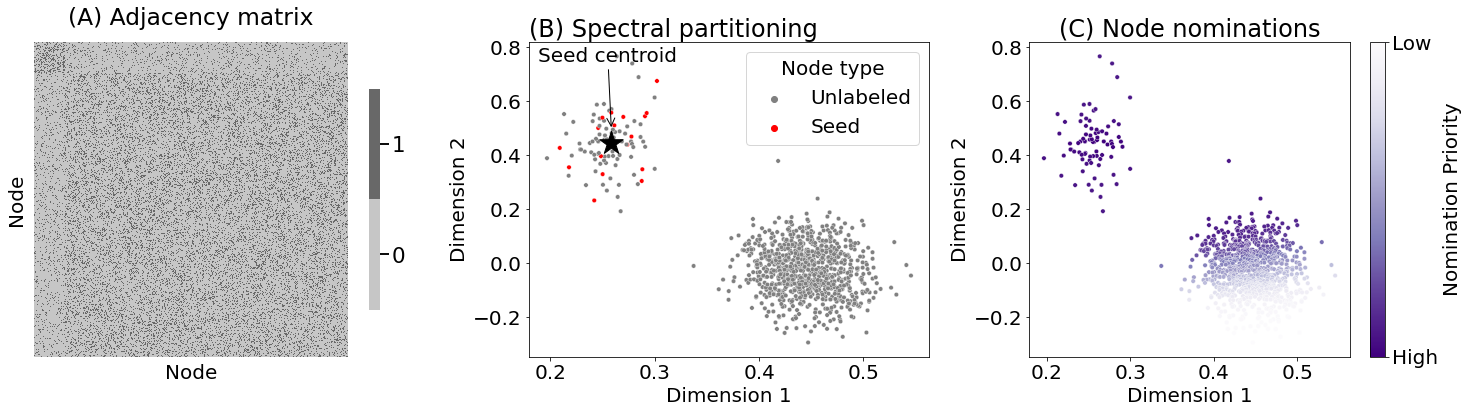
\includegraphics[width=\linewidth]{applications/ch7/Images/vn.png}
    \caption[Web page network for vertex nomination.]{\textbf{(A)} The adjacency matrix for the web page network. \textbf{(B)} the estimated latent positions for the nodes in the web page network (faint points). The centroid of the seed nodes is annotated directly. \textbf{(C)} the nomination priorities for each of the unlabelled nodes. Nodes which are closer to the seed centroid have higher priority.}
    \label{fig:ch7:vn:ex}
\end{figure}

Back in Section \ref{sec:ch6:ase}, we used the Euclidean distance from Remark \ref{def:ch6:se:eucl_dist} to quantify what we meant by nodes from the same community having ``similar'' estimated latent positions. Remember that when we used \texttt{KMeans} to estimate the unknown community assignments in Section \ref{sec:ch7:comm_detect}, the key idea was that we could exploit the fact that nodes in the same community had similar latent positions to identify clusters of nodes which had similar latent positions. This resulted in community-specific mean vectors $\vec \mu_k$, and we assigned points to communities depending on their proximity to the community-specific mean vectors.

Here, we will use a similar insight. We already know the community assignments for the seed vectors in our community of interest, and all nodes $i$ from the same community have the same underlying latent position $\vec x_i$. This property does not hold in the estimated latent positions $\hat{\vec x}_i$ for the nodes in the same community, since the latent positions are imperfectly estimated, which we learned from Section \ref{sec:ch6:ase}.

Since the underlying latent positions of the random network are the same, a reasonable estimated latent position for the community can be obtained by performing a spectral clustering (via \texttt{KMeans}, like we did in Section \ref{sec:ch7:comm_detect}):

\begin{lstlisting}[style=python]
from graspologic.embed import AdjacencySpectralEmbed as ase
from sklearn.cluster import KMeans
from graphbook_code import ohe_comm_vec

Xhat = ase().fit_transform(A)
# community detection with kmeans
km_clust = KMeans(n_clusters=2)
km_clust.fit(Xhat)
labels_kmeans = km_clust.fit_predict(Xhat)
\end{lstlisting}

For each seed node, we can obtain the a surrogate for the estimated latent position associated with the community of the seeds by simply finding which of the communities the seeds tended to be assigned to, and then using the centroid associated with this community to find nodes most similar to the seed nodes:

\begin{lstlisting}[style=python]
# estimated community assignment matrix
Chat = ohe_comm_vec(labels_kmeans)

# get the community (class) with the most seeds
comm_of_seeds = np.argmax(Chat[seed_ids,:].sum(axis=0))

# get centroid of the community that seeds tend to be
# assigned to
centroid_seeds = km_clust.cluster_centers_[comm_of_seeds]
\end{lstlisting}

The centroid of the community that the most seed nodes were assigned to is indicated in Figure \ref{fig:ch7:vn:ex}(B), by the large red star. 

Finally, using the Euclidean distance, we can estimate the spatial proximity for each unlabeled node to the centroid that the most the seed nodes were assigned to. We will use this spatial proximity to the centroid as a surrogate for unlabeled nodes being ``similar'' to the seed nodes in producing our nomination list:

\begin{lstlisting}[style=python]
from scipy.spatial.distance import cdist
from scipy.stats import rankdata

# compute the distance to the centroid for all estimated latent positions
dists_to_centroid = cdist(Xhat, centroid_seeds.reshape(1, -1)).reshape(-1)
# compute the node numbers for all the nonseed nodes
nonseed_bool = np.ones((np.sum(ns)))
nonseed_bool[seed_ids] = 0
nonseed_ids = np.array(np.where(nonseed_bool)).reshape(-1)

# isolate the distances to the centroid for the nonseed nodes
nonseed_dists = dists_to_centroid[nonseed_ids]
\end{lstlisting}

To produce the nomination list, we can sort the distances of the nonseed nodes to the centroid, return the index-sorted ordering, and then output our nomination list by using reordering the nonseed indices in order of their distances. The following code will do just this for us:


\begin{lstlisting}[style=python]
# produce the nomination list
nom_list_nonseeds = np.argsort(nonseed_dists).reshape(-1)
# obtain a nomination list in terms of the original node ids
nom_list = nonseed_ids[nom_list_nonseeds]
\end{lstlisting}

In Figure \ref{fig:ch7:vn:ex}(C), we color the unlabeled nodes (which were gray in Figure \ref{fig:ch7:vn:ex}(B)) by their spatial proximity to the seed centroid. Note that the unlabelled nodes which are closest to the seed centroid tend to have higher spatial proximities, and are hence higher priority in the nomination list (with a smaller numerical label in \texttt{nom\_list}).

This procedure is known as the ``Spectral Partitioning Nomination Scheme'', or \texttt{sp}, and has been studied in several areas of application \cite{Fishkind2015Sep,Yoder2018Feb}.

\subsection{Extensions to other problems}

There are a large number of ways that we could have approached the vertex nomination problem differently. Let's take a look at a few of them.None of these approaches are ``better'' or ``worse'', than others, and it is important to highlight that each can be leveraged to answer a different network learning question \cite{Coppersmith2012Jan,Coppersmith2014Mar,Yoder2018Feb,Fishkind2015Sep,Fishkind2019Mar}. When you have a vertex nomination problem, you will likely have to tailor the strategy to your network data.


\paragraph*{Different strategies for spectral partitioning}

We presumed that our network had two communities, and two embedding dimensions, which was largely a function of visual simplicity when viewing the node nominations in Figure \ref{fig:ch7:vn:ex}(C). However, there is no reason we need to necessarily assume the number of communities or the ahead of time, and we could just as easily have used dimensionality selection as in Section \ref{sec:ch6:dimest:dimselect}, automated the community selection procedure like we did in Section \ref{sec:ch7:comm_detect}, or substituted different clustering algorithms and different notions of similarity.

For instance, a popular choice for community detection in \cite{Yoder2018Feb} is \texttt{GMM}, where the notion of similarity is the probability density of a particular unlabeled point given the mean and variance of the cluster the most seeds are assigned to. This enables robustness to networks where the underlying random network is $DCSBM_n(\vec z, \vec \theta, B)$, which you learned in Section \ref{sec:ch7:comm_detect}.

\paragraph*{Extending spectral partitioning to related problems}

The spectral partitioning nomination scheme can be extended directly to many other related problems. A key limitation here is that we are presuming that our nodes are in one of two groups, and all of the labeled nodes that we pass in are associated with the same group. Our goal is to prioritize nodes that are likely to also be from that same group. 

On the other hand, we could have just as easily identified nomination lists on a per-seed-node basis; e.g., for each seed node, we could have found a set of unlabeled nodes that have spatially proximal estimated latent positions. This extension provides the intuitive foundation for the \textit{graph matching problem} \cite{Fishkind2015Sep, Fishkind2019Mar}, which you will learn about in Section \ref{sec:ch8:gm}.

\paragraph*{We could have ignored partitioning techniques entirely}

We could have ignored partitioning and latent community detection approaches entirely, and simply estimated the ``centroid'' directly by taking the average estimated latent position of all of the seed nodes.

\newpage